\chapter{On the Use of Doppler to Enrich Obstacle Avoidance}
To ensure more safe trajectories for social indoor environments we can use velocity information from targets to generate more safe pathing for  the robot. Although we have not completed it entirely  we tried to create a software module that takes this objective in mind.

In this section we will explore the implementation of a new plugin in the ROS navigation stack based on the radar's relative radial velocity information. The plugin proposed is a map layer and can be specified by either the global or local costmap. The objective of said layer is to increase the cost values of cells based on the prediction of the motion of said obstacles provided by the radar (doppler channel). The ending result should be a better avoidance of incoming obstacles with negative relative velocity  to the robot.

\section{Layered Costmaps}
As said before the global and local costmaps used in \ac{ROS} Navigation Stack are both layered costmaps.
This means that they are composed by independent components with each one affecting the resulting master layered costmap for specific environmental contexts. For example the classic \textit{static layer} takes information from a published map topic and based on the position of the robot marks some  pre-determined obstacles while the inflation layer propagates the cost of obstacles radially.  Figure \ref{fig::layers} show some different layers for different contexts.
\begin{figure}[ht!] 
\centerline{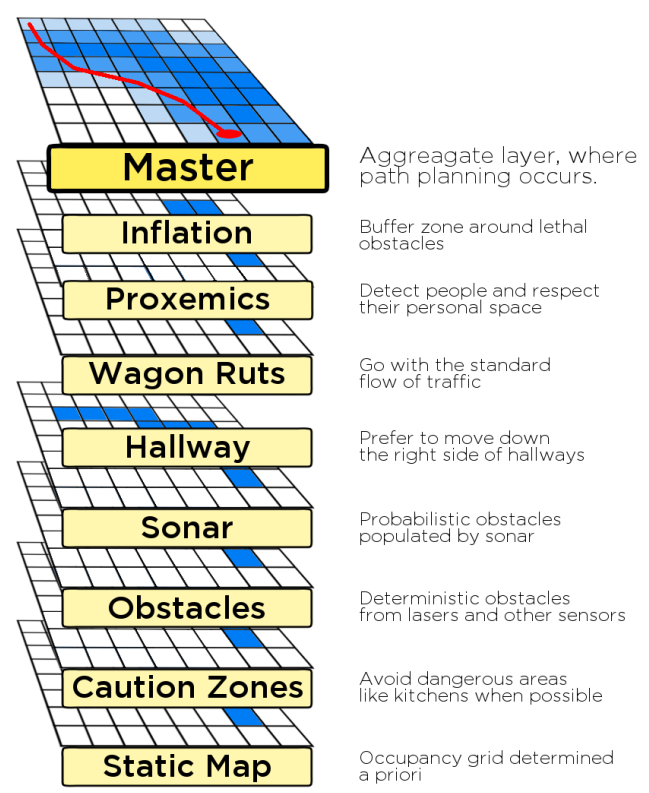
\includegraphics [width=0.5 \textwidth]{imgs/chapter6/layers.png}}
\caption[A stack of costmap layers]{A stack of costmap layers, showcasing the different contextual
behaviors achievable with the layered costmap approach from \cite{lu2014layered}}
\label{fig::layers}
\end{figure}

The set of layers used follows a specific hierarchy that determines what order and how they overwrite the master costmap. This is an important part to take into consideration because the priority of the different layer plugins will determine the final costmap that will be used by each planner (global or local).
\section{Inflation Layer}
When it comes to define values for the costmap occupancy grid the inflation layer is usually the case in the \ac{ROS} navigation stack. By definition, inflation is the process of propagating cost values out from occupied cells that decrease with distance \cite{costmap2d}. Figure \ref{fig::inflation} shows an overview of the different values each cell can have (0 to 254) and what they mean when it comes to the robot perception. 
\begin{figure}[ht!] 
\centerline{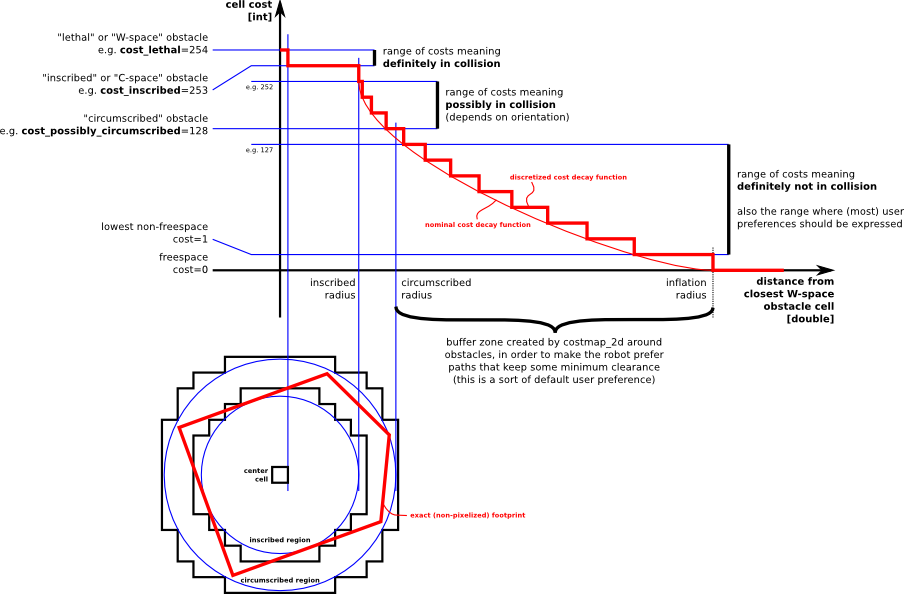
\includegraphics [width=1.0 \textwidth]{imgs/chapter6/costmapspec.png}}
\caption{Inflation layer specifications from \cite{costmap2d}}
\label{fig::inflation}
\end{figure}

All cells in the costmap further than the inscribed radius distance and closer than the inflation radius distance away from an actual obstacle is given by:
\begin{equation}
    A=253*e^{(-k * (dist - r)) }
\end{equation}
Where $k$ is the cost scaling factor  that determines how fast the decaying of the function is, $dist$ is the distance from the obstacle to the robot and finnaly $r$ is the robot radius. 
This means that cells near obstacles will have the value that will tend to 253 while cells far away from the obstacle will have values trending to 0. Note that $dist$ most be always greater than $r$ because if it isn't than it means the robot collided with said obstacle.
This inflation is only taking into account distance from the obstacle as input which means that the values of the cells will be propagated radially.

\section{Doppler Layer}
In the previous case, inflation only took into account the distance of obstacles for computing what value each cell in the costmap will have. Now we want to design a layer that not only takes into account the distance but also the relative radial velocity of the object to determine the value of cells in the costmap.
To do this we designed a layer that adjusts the cell values of the master costmap taking into account the radial velocity of said objects taken from the \ac{FMCW} \ac{radar}. Taking into account the relative  radial velocity $v_r$ the cell value of the surrounding cell's is given by:
\begin{equation} \label{eq1}
\begin{split}
cell_{cost} & = A e^{-(\frac{x^2}{2 \sigma_x^2}+\frac{y^2}{2 \sigma_y^2})} \\
 \sigma_x^2 & = cov * factor * |v_r| \\
 \sigma_y^2 & = cov \\
 x & =dist *cos(\theta)\\
 y & =dist *sin(\theta)\\
\end{split}
\end{equation}
Where $cov$ and $factor$ are parameters adjusted by the user, $\theta$ is the angle between the cell where we want to calculate its value and the direction of the velocity vector of the target object, and finally $dist$ is the distance between the two previous cells.
With this cost function we can manipulate the costmap cell values to have higher values in the directon of incoming objects. Figure \ref{fig::doppler} shows an example of the doppler layer changing the 2D master costmap taking into account the velocity and distance of the target obstacle. 

\begin{figure}[h] 
\centerline{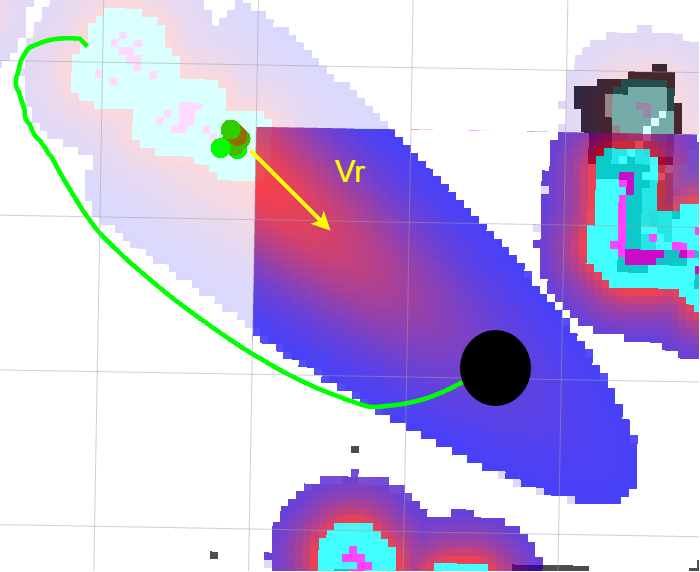
\includegraphics [width=1.0 \textwidth]{imgs/chapter6/doppler.png}}
\caption[Doppler layer manipulation of the master costmap]{Example of doppler layer manipulation of the master costmap with the paramaters  A=253,factor=20 and covariance=0.1}
\label{fig::doppler}
\end{figure}
\section{Discussion}
By using the doppler layer we have concluded that the trajectory of the robot can be altered taking into consideration the relative radial velocity of the target obstacles. This may be useful for high populated indoor environments where people constantly are shifting from one place to another. This makes the robot safe from incoming obstacles and therefore is a good support for our navigation system. There are some limitations for this layer however, the first one being that the velocity resolution of the radar is limited which may produce bad results when the radial velocity of the objects is low. Another limitation is that the global costmap update is usually around 1 Hz, and alot of information may be outdated when the control loop occurs which may lead on late replanning by the global planner. For the local planner another problem is its limited dimensions do not allow the prediction of long range obstacles since it only works in the vicinity of the robot.
%\section{Summary}
%In this chapter we discussed how we can implement a new layer to manipulate the master costmap of the global and local planners. This layer inflates obstacles in the direction of their velocity. Since we have radial relative velocity of points given by the radar we can use their velocities to compute a safe path for the robot.


%\subsection{Side Tracking}

%\subsection{Target Speed Limitations}

%\section{Summary}